\section{Interpretation der Ergebnisse}
\label{sec:04_dokumentation_interpretation_ergebnisse}

Beide Modelle wurden nicht mittels einer Gridsearch optimiert, da durch die
sukzessive Veränderung der Daten eine aufwendige Suche der optimalen Parameter
notwendig wäre.
Stattdessen wurde der Fokus auf robuste Modelle gelegt, die 
resistent gegen den Mismatch in den Daten sind.

Der Random Forest erweist sich bei kleinen Datensätzen und sehr großem
Mismatch \SI{30}{\percent} als zuverlässigeres Modell.
Trotz des Missmatch betrug die Accuracy \SI{50}{\percent}. 
Dies lässt sich darauf zurückführen, dass der Mismatch mit der relativen
Häufigkeit der Klassen korreliert ist. 
Zu den häufigsten Klassen zählen die Klassen \textit{keine Wolken}, 
\textit{Stratocumulus} und \textit{Nimbostratus}. 
Diese weisen alle ein charakteristisches Farbspektrum auf und sind einfach
anhand dessen von den anderen Klassen zu trennen.
Das Training des CNN dagegen stellte sich als schwierig heraus. 
Trotz verschiedener Kernel-Größen und Anzahl an Convolutional Schichten ließ
sich die Accuracy nicht wesentlich über \SI{30}{\percent} anheben. 
Denkbar wäre gewesen, auf die Convolution zu verzichten und ebenso wie beim
Random Forest auf dem Farbspektrum zu trainieren.
Diese Methode erschien wesentlich einfacher zu regularisieren um den Missmatch
zu handeln.
Die Entscheidung fiel jedoch bewusst dagegen aus, um das Verhalten des Neuronalen Netzes
auf schlecht simulierten Daten zu studieren. 

\begin{wrapfigure}{r}{0.6\textwidth}
		\vspace{-0.6cm}
		\centering
		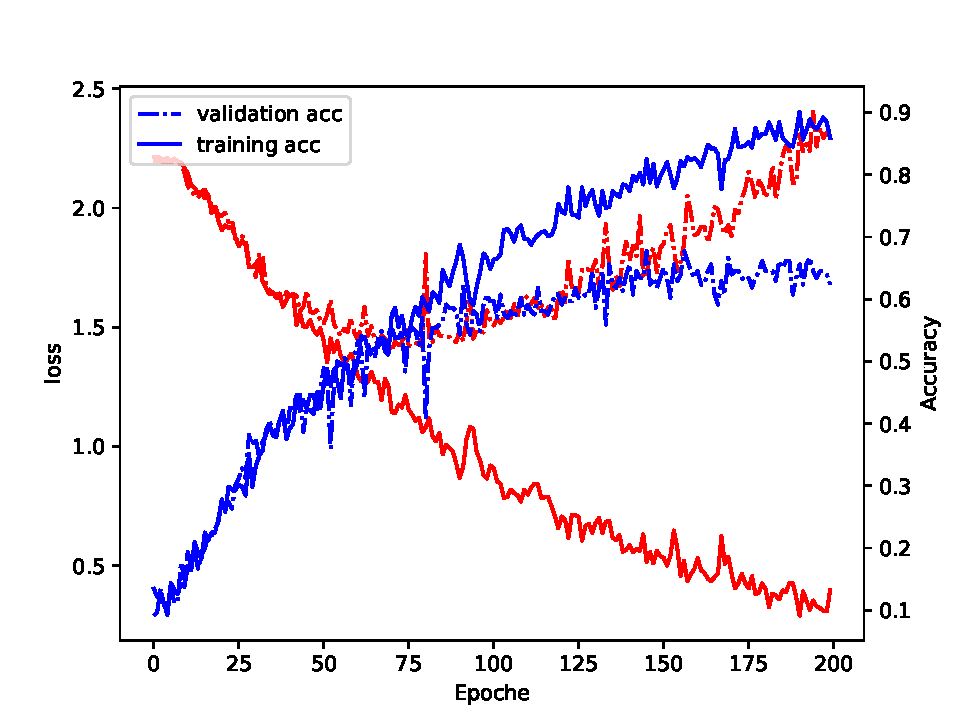
\includegraphics[width=0.6\textwidth]{pictures/train_nn.pdf}
		\vspace{-1.2cm}
		\caption{Loss sowie Accuracy in Abhängigkeit der Trainings Epochen für
		Trainings sowie Validierung Daten.}
		\vspace{-0.2cm}
		\centering
		\label{fig:t_nn}
\end{wrapfigure}
Der Random Forest erreicht auf dem finalen Datensatz, der immer noch einen
kleinen Missmatch enthält, aus der Uneindeutigkeit der Klassen und dem Fehler
des Bots eine Accuracy von \SI{75}{\percent}. 
Auf dem selben Test-Datensatz zur Evaluation beträgt die Accuracy des CNN ca
\SI{65}{\percent}.
Dabei ist die Accuracy abhängig, bei welcher Epoche der Schnitt zwischen Over-
und Underfitting macht.
Trotz einer Trainingszeit von über acht Stunden scheint das Netz noch nicht zu
Übertraining zu neigen, da weder der Validation Loss trotz des 
Missmatch Problemes auffällig steigt, noch die Validation Accuracy 
sinkt (vergleiche Abbildung \ref{fig:t_nn}).
Ein wesentlich schnelleres Training konnte auch nicht durch das verwenden 
anderer Loss Funktionen und Learningrates erreicht werden.
In Abbildung \ref{fig:conf} sind die Confusion Matrizen der beiden Modelle
dargestellt. 
\begin{figure}[h]
		\centering
		\begin{subfigure}[b]{0.49\textwidth}
				\begin{center}
						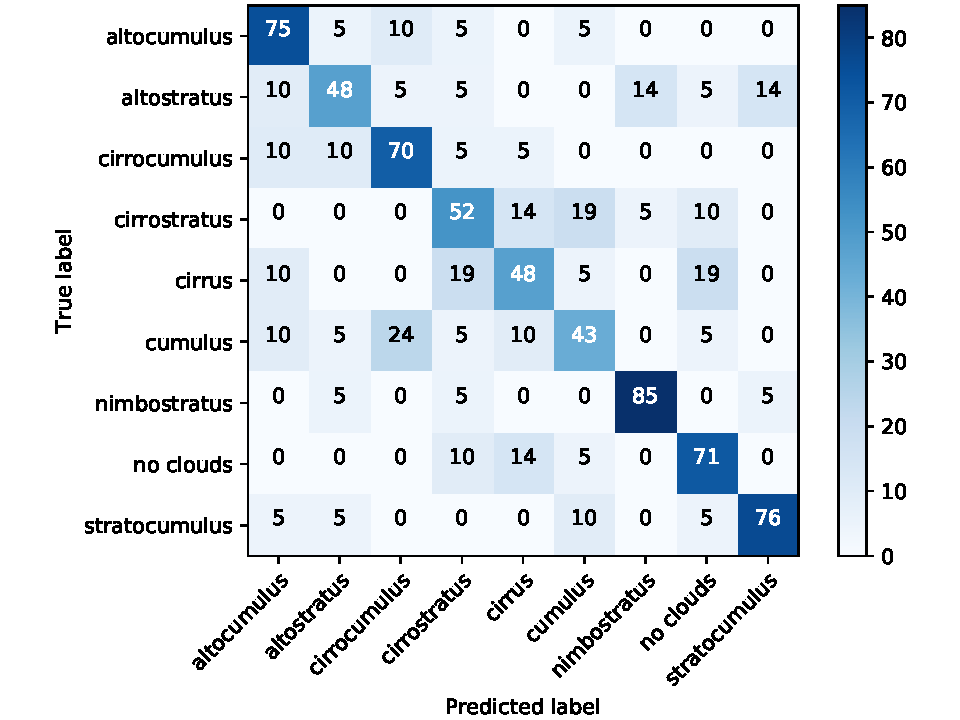
\includegraphics[width=\textwidth]{./pictures/conf_rf.pdf}
				\end{center}
		\vspace{-0.6cm}
				\caption{Random Forest}
				\label{fig:conf_rf}
		\end{subfigure}
		\begin{subfigure}[b]{0.49\textwidth}
				\begin{center}
						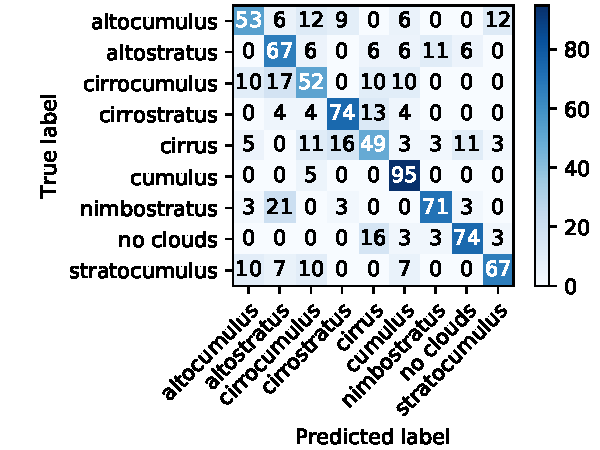
\includegraphics[width=\textwidth]{./pictures/conf_nn.pdf}
				\end{center}
		\vspace{-0.6cm}
				\caption{Convolutional Neuronal Network}
				\label{fig:conf_cnn}
		\end{subfigure}
		\caption{Konfidenz Matrizen der observierten Klassen bei denen das
		Vorhergesagte gegen das Wahre Klasse aufgetragen ist.}
		\label{fig:conf}
\end{figure}
Prinzipiell scheinen beide Modelle jeweils Probleme zu haben, wenn das 
Farbspektrum zweier Klassen sich nicht wesentlich unterscheidet.
Dies ist überwiegend dann der Fall, wenn die Wolkenbedeckung des Himmels sich
flächenmäßig ähnelt. 
Trotz einer niedrigen gesamten Accuracy scheint das CNN einen 
Erkenntnisgewinn aus den Kanten der Cumuluswolken zu ziehen, da die Accuracy
der Klasse höher ist, als beim Random Forest.
Dies ist erfreulich, da dies als ein Hinweis darauf, dass das CNN 
die Kanten der Wolken interpretieren kann, angesehen werden kann. 

\begin{wrapfigure}{l}{0.32\textwidth}
		\centering
		\vspace{-0.4cm}
		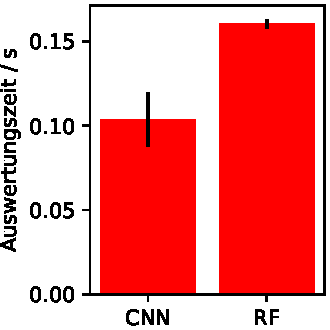
\includegraphics[width=0.3\textwidth]{pictures/time.pdf}
		\caption{Auswertung zeit auf Test Daten.}
		\label{fig:time}
		\vspace{-0.5cm}
\end{wrapfigure}
Der beschränkende Faktor beim Training des CNN ist einerseits die hohe
Trainingszeit, welches die Suche nach den besten Einstellung schwierig macht da, 
diese lange zum Trainieren brauchen und andererseits die sehr
beschränkte Größe des Datensatzes. 
Der Mismatch der Daten scheint die Methoden zwar zu beschränken aber dennoch
ein akkurates Ergebnis zu ermöglichen.
Die Auswertungszeit des CNN ist geringer als beim Random Forest (siehe Abbildung
\ref{fig:time}). 
Dadurch lässt sich die Triggerrate mit denen Wolken klassifiziert werden
erhöhen.
Es werden keine Plots zur Confidence Verteilung der einzelnen Klassen erstellt,
da bei einer Live-Analyse Confidence Schnitte auf den Vorhersagen zu dem 
sporadischen nicht Kategorisieren einer Wolke führen würden.
Dadurch würden Lücken in der zeitlichen Observation der Wolkenbedeckung
entstehen.
